% $HeadURL: https://sbgn.svn.sourceforge.net/svnroot/sbgn/ProcessDiagram/tags/L1V1.3Full/sources/complex-epn-eg.tex $

\subsection{Examples of complex EPNs}
\label{sec:CplxEPNs}

In this section, we provide examples of Entity Pool Node representations drawn using the \SBGNPDLone glyphs described above. 

\fig{example-camkii} represents calcium/calmodulin kinase II, with phosphorylation on the sites threonine 286 and 306, as well as catalytic and autoinhibitory domains.  Note the use of \emph{units of information} and \emph{state variables}.

\begin{figure}[H]
  \centering
  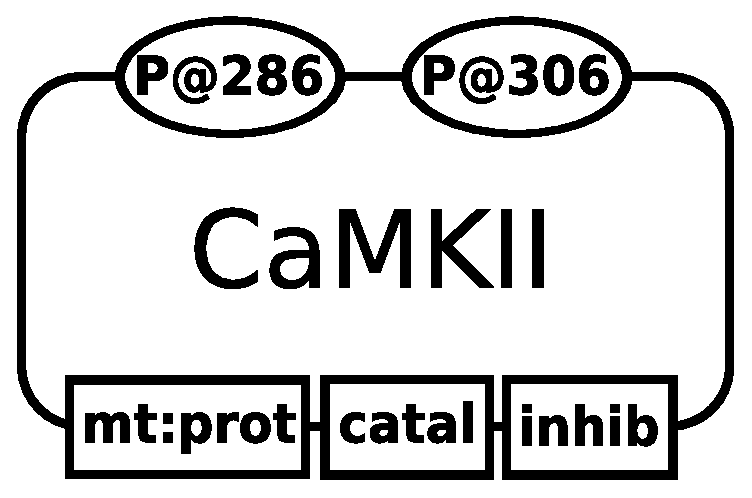
\includegraphics[scale = 0.3]{examples/macromolecule-CaMKII}
  \caption{An example representation of calcium/calmodulin kinase II.}
  \label{fig:example-camkii}
\end{figure}

\fig{example-glur} represents the glutamate receptor in the open state, with both phosphorylation and glycosylation.  The entity carries two functional domains, the ligand-binding domain and the ion pore, and its chemical nature is precided.

\begin{figure}[H]
  \centering
  \includegraphics[scale = 0.3]{examples/macromolecule-GluR}
  \caption{An example of a glutamate receptor in the open state.}
  \label{fig:example-glur}
\end{figure}




%%% Local Variables: 
%%% mode: latex
%%% TeX-master: "../sbgn_PD-level1"
%%% End: 
